% Draft v1.0 -- Team Transmontane
% Based on the official CVPR author kit (https://github.com/cvpr-org/author-kit)
% Upload this whole folder to Overleaf (New Project -> Upload Project -> zip of this folder)
% Compiler: pdfLaTeX, main document: main.tex

\documentclass[10pt,twocolumn,letterpaper]{article}

%%%%%%%%% PAPER TYPE
% \usepackage{cvpr}              % camera-ready
% \usepackage[review]{cvpr}      % anonymous review version (switch to this before submitting!!)
\usepackage[pagenumbers]{cvpr}   % draft with names + page numbers, for internal review

%% This file contains a number of tweaks that are typically applied to the main document.
%% They are not enabled by default, but can be enabled by uncommenting the relevant lines.


%%
%% Official support for 2-column teaser figure
%%
\usepackage{cuted} %< for strip environment

%%
%% For auto-referencing of figures (see fig/teaser.tex and \label{} therein) 
%%
\usepackage{currfile} %< for \currfilebase macro

%%
%% caption and (global) spacing overrides
%%
\usepackage{caption} %< for "\captionof" commands (teaser)
% \setlength{\abovecaptionskip}{.5em} % space above caption
% \setlength{\belowcaptionskip}{1em} % space below caption

%%
%% Inline annotations; for predefined colors, refer to "dvipsnames" in the xcolor package:
%% https://tinyurl.com/overleaf-colors
%%
\newcommand{\red}[1]{{\color{red}#1}}
\newcommand{\todo}[1]{{\color{red}#1}}
\newcommand{\TODO}[1]{\textbf{\color{red}[TODO: #1]}}
%%
%% Disable for camera ready / submission by uncommenting these lines:
%%
% \renewcommand{\TODO}[1]{}
% \renewcommand{\todo}[1]{#1}

%%
%% Work harder in optimizing text layout. Typically shrinks text by 1/6 of page, enable
%% it at the very end of the writing process, when you are just above the page limit.
%%
% \usepackage{microtype}

%%
%% Fine-tune paragraph spacing.
%%
% \renewcommand{\paragraph}[1]{\vspace{.5em}\noindent\textbf{#1.}}

%%
%% Globally adjusts space between figure and caption.
%%
% \setlength{\abovecaptionskip}{.5em}

%%
%% Allows "the use of \paper to refer to the project name"
%% with automatic management of space at the end of the word.
%%
% \usepackage{xspace}
% \newcommand{\paper}{ProjectName\xspace}

%%
%% Commonly used math definitions.
%%
% \DeclareMathOperator*{\argmin}{arg\,min}
% \DeclareMathOperator*{\argmax}{arg\,max}

%%
%% Tighten underline.
%%
% \usepackage{soul}
% \setuldepth{foobar}

%%
%% Reconfigure paragraph (tweaks spacing)
%%

\usepackage{multirow}
\usepackage{makecell}
\usepackage{pifont}
\newcommand{\cmark}{\ding{51}}
\newcommand{\xmark}{\ding{55}}

\definecolor{cvprblue}{rgb}{0.21,0.49,0.74}
\usepackage[pagebackref,breaklinks,colorlinks,allcolors=cvprblue]{hyperref}

\def\confName{CVPR}
\def\confYear{2027}

% our own short-hands
\newcommand{\gdino}{Grounding DINO\xspace}
\newcommand{\lae}{LAE-80C\xspace}
\newcommand{\std}{\textsc{std}\xspace}
\newcommand{\src}{\textsc{src}\xspace}

%%%%%%%%% TITLE
% HR: title agreed in the meeting, Saurav's "Less is more ..." sounded too clickbait
\title{Choosing What to Look For: Adaptive Per-Image Vocabulary Selection for Open-Vocabulary Object Detection in Aerial Imagery}

%%%%%%%%% AUTHORS
\author{Amit Adhikari \qquad Himanshu Ray \qquad Saurav Kumar Gupta \qquad Avishek Chowdhury\\
Team Transmontane
% add department, university and emails here for the camera-ready version
% (the [review] version is anonymous, so this block is not printed there)
}

\begin{document}
\maketitle

% AC: abstract written last night, numbers are from FINAL_TEST.md, pls dont change them without checking the metrics json
\begin{abstract}
Open-vocabulary detectors like \gdino can detect any class that is written in the text prompt, but on aerial images giving the detector a long list of fine-grained and overlapping class names make the accuracy collapse almost to zero.
In this work we ask a simple question, can we choose a small vocabulary for every image \emph{before} detection, without any training, so that a frozen detector works better?
We propose a training-free selector that score all 80 candidate classes with the remote sensing CLIP model RemoteCLIP and keeps every class whose probability is above a threshold calibrated once on held-out images, so the size of vocabulary adapt to each image (around 8 classes on average).
The selector only see the pixels and cost about 8\,ms per image.
We evaluate on \lae with a source-aware protocol that account for its five disjoint label spaces, all our choices were frozen before a single run on 2,862 held-out test images.
The selector raise AP50 of \gdino-T from 0.0053 to 0.0280 under standard COCO scoring and from 0.0157 to 0.0418 under source-aware scoring, both robust under three statistical checks, and it is also 1.21$\times$ faster end-to-end.
However the gain is mostly on imagery similar to the encoder's training data (DIOR/DOTA, and NWPU VHR-10 without retuning) and it disappear on FAIR1M and xView.
\TODO{one more line on negative results? maybe drop if over length}
\end{abstract}

\section{Introduction}
\label{sec:intro}

\begin{figure*}[t]
  \centering
  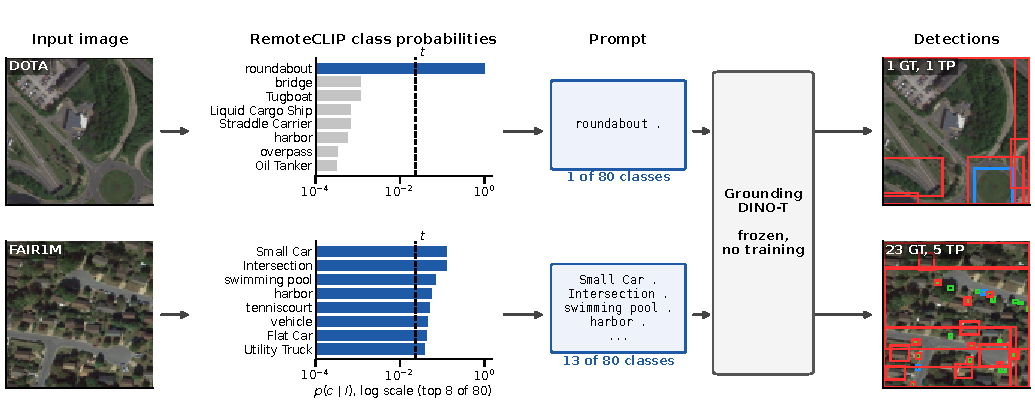
\includegraphics[width=\textwidth]{fig/pipeline.pdf}
  \caption{Overview of our training-free selector on two real dev images. RemoteCLIP turns the pixels into a probability for each of the 80 class names, and every class above the calibrated threshold $t$ (dashed line) goes into the prompt of the frozen detector. A confident image (top, DOTA roundabout) keeps a single class, an ambiguous residential scene (bottom, FAIR1M) keeps 13. Blue bars are kept classes; only the 8 most probable classes are drawn. In the output panels green boxes are ground truth, blue are true positives and red are false positives at score $\geq0.14$.}
  \label{fig:pipeline}
\end{figure*}

Open-vocabulary object detection (OVD) lets the user decide at test time which classes the detector should look for, simply by writing their names \cite{liu2024grounding}.
For natural images this works surprisingly well.
Remote sensing imagery is a different story.
Aerial images contain many small and densely packed objects seen from the top, and the class lists of remote sensing benchmarks are long and full of near duplicates.
\lae \cite{pan2025lae}, for instance, contains \emph{vehicle}, \emph{small car}, \emph{passenger car} and \emph{van} at the same time.
When all such names are put in one prompt, the detector has to divide its confidence among look-alike names and the result is very poor: LAE-DINO \cite{pan2025lae} reports only 0.1 mAP for a \gdino-T pretrained on natural images.

The text prompt is not a passive filter in these models.
In \gdino the class names enter the feature enhancer, the query selection and the decoder, so they change the visual features themselves \cite{liu2024grounding,fu2026wedetect}.
Work on natural images also shows that the class text steers box regression, so a wrong name can pull the box onto the wrong object \cite{wang2023condhead}, and that overlapping concepts split the probability mass of a classifier \cite{li2024lbp}.
A long vocabulary also costs time, because a fusion detector has to run its text--image fusion again for every chunk of the prompt (31 passes for the 1,203 LVIS classes in \cite{fu2026wedetect}).
Hence, for a frozen detector, choosing the vocabulary is the main control that the user still has over the output.

How much does it matter on aerial data?
A recent zero-shot study \cite{tsourveloudis2026ovd} found that prompting \gdino with only the ground-truth classes of each \lae image raises F1 by about 15$\times$, and it lists vocabulary filtering as an open direction.
That number comes from an oracle that reads the labels, so it shows the headroom but it is not something one can deploy.

The natural next step is to look at the image first, guess which classes are present, and prompt the detector with only those.
The idea by itself is not new.
VocAda \cite{liu2025vocada} adapts the vocabulary per image at test time with a captioner (LLaVA-Next-7B), a noun parser and a class selector, and reports consistent gains on COCO and Objects365.
However it was tested on natural images with Detic-style detectors, and it costs 5.6--10.7\,s and 17--31\,GB of GPU memory per image \cite{liu2025vocada}.
That is not practical for large aerial archives, and it does not even fit on the 8\,GB GPU we had.
SHiNe \cite{liu2024shine} and the fine-grained benchmark of Bianchi \etal \cite{bianchi2024devil} show from other angles that OVD detectors are sensitive to how the vocabulary is written and that they degrade when it contains irrelevant or hard-negative entries.
In our literature search (last repeated in October 2026) we could not find any study of a cheap, deployable per-image selector for a \emph{frozen} OVD detector on \emph{aerial} imagery.

In this work we build such a selector and we have tried to be careful with the evaluation, because early in the project we noticed that the benchmark itself has a trap.
\lae merges five source datasets that annotate \emph{disjoint} sets of classes, so a correct ``vehicle'' box on a FAIR1M image (where cars are labelled ``Small Car'') is counted as a false positive by standard COCO evaluation.
We therefore report a source-aware score next to the standard one, decided before any test run.
Our selector (\cref{fig:pipeline}) uses RemoteCLIP \cite{liu2024remoteclip} to score all 80 names from the pixels and keeps every name above one calibrated threshold, so a clear image gets a very short prompt and an ambiguous one gets a longer prompt.

Our contributions are as follows.
\begin{itemize}
    \item A training-free, pixels-only selector that picks a per-image vocabulary with RemoteCLIP and an \emph{adaptive} size controlled by a single calibrated threshold. It adds about 8\,ms per image and needs no change to the detector.
    \item An evaluation protocol for merged benchmarks: source-aware AP, a difference that is called robust only when a percentile bootstrap, a basic bootstrap and a per-class sign test all agree, and a test split that was used exactly once after every choice was frozen.
    \item On 2,862 held-out test images the selector improves AP50 by 5.3$\times$ (standard) and 2.7$\times$ (source-aware) over the full 80-class prompt, beats a fixed top-8 selector built on the same encoder, and makes the pipeline 1.21$\times$ faster.
    \item A clear map of where this works and where it does not. The gain holds on DIOR/DOTA-like data and transfers to NWPU VHR-10 \cite{cheng2014nwpu} untuned, but it is absent on FAIR1M and xView. Several extensions that we expected to help (crop evidence, uncertainty-aware retention, captions, synonym expansion) did not improve detection, and we report them as negative results.
\end{itemize}

\section{Related Work}
\label{sec:related}

\begin{table}[t]
  \centering
  \small
  \setlength{\tabcolsep}{3.2pt}
  \begin{tabular}{@{}lccccc@{}}
    \toprule
    Method & Venue & \makecell{No\\training} & \makecell{Frozen\\detector} & \makecell{Per-image\\vocab.} & Aerial \\
    \midrule
    Rasheed \etal \cite{rasheed2022bridging} & NeurIPS'22 & \xmark & \xmark & \xmark & \xmark \\
    CondHead \cite{wang2023condhead} & CVPR'23 & \xmark & \xmark & \xmark & \xmark \\
    LBP \cite{li2024lbp} & CVPR'24 & \xmark & \xmark & \xmark & \xmark \\
    GenerateU \cite{lin2024generateu} & CVPR'24 & \xmark & \xmark & n/a$^a$ & \xmark \\
    WeDetect \cite{fu2026wedetect} & CVPR'26 & \xmark & \xmark & \xmark & \xmark \\
    SHiNe \cite{liu2024shine} & CVPR'24 & \cmark & \cmark & \xmark & \xmark \\
    VocAda \cite{liu2025vocada} & ICIP'25 & \cmark & \cmark & \cmark & \xmark \\
    CastDet \cite{li2024castdet} & ECCV'24 & \xmark & \xmark & \xmark & \cmark \\
    LAE-DINO \cite{pan2025lae} & AAAI'25 & \xmark & \xmark & train$^b$ & \cmark \\
    OpenRSD \cite{huang2025openrsd} & ICCV'25 & \xmark & \xmark & \xmark & \cmark \\
    Tsourveloudis \cite{tsourveloudis2026ovd} & arXiv'26 & \cmark & \cmark & oracle$^c$ & \cmark \\
    \midrule
    \textbf{Ours} & & \cmark & \cmark & \cmark & \cmark \\
    \bottomrule
  \end{tabular}
  \caption{Where our work sits. ``Per-image vocab.'' means the class list is changed per image at test time. $^a$Names are generated, no list is used. $^b$Vocabulary is sampled per batch during training only. $^c$Ground-truth classes, used as an upper bound.}
  \label{tab:position}
\end{table}

\cref{tab:position} places our work among the methods discussed below.

\paragraph{Open-vocabulary detection.}
Most two-stage OVD detectors align region features with a frozen vision-language embedding space and then classify regions against the text embeddings of the class names \cite{radford2021clip}, \ie the classifier weights are replaced by the embedded vocabulary \cite{rasheed2022bridging}.
Training-based improvements in this family are many.
Rasheed \etal \cite{rasheed2022bridging} make CLIP features object-centric by region distillation and by pseudo-boxes from image-level labels, and they show how much the proposal source matters (novel AP50 of 4.0 with RPN proposals against 16.7 with MViT proposals in the same setting).
LBP \cite{li2024lbp} learns prompts for the unnamed objects hidden in the background class, CondHead \cite{wang2023condhead} conditions the box and mask heads on the class embedding and gains 3.0 APr on LVIS for about 1\% more FLOPs, and Zhao \etal \cite{zhao2024samp} learn scene-adaptive and region-aware prompts.
\gdino \cite{liu2024grounding} instead fuses image and text deeply, so the whole class list goes into one BERT \cite{devlin2019bert} prompt of at most 256 tokens.
WeDetect \cite{fu2026wedetect} goes the other way and drops fusion completely, treating detection as retrieval against cached text embeddings, which makes it about ten times faster than \gdino-T.
GenerateU \cite{lin2024generateu} removes the class list altogether and generates a name for every box.
All of these need training on detection or grounding data, from base-class fine-tuning up to 15M images for WeDetect.
We take \gdino-T as it is and never update it.

\paragraph{The vocabulary as a source of errors.}
Several works show that the vocabulary itself changes the result a lot.
SHiNe \cite{liu2024shine} finds that accuracy varies with the granularity of the class names and that adding 1,466 unrelated ``noisy'' classes drops its baseline by about 4 mAP50.
Bianchi \etal \cite{bianchi2024devil} build per-object vocabularies of hard negatives that differ in one attribute and find that detectors that do well on COCO/LVIS cannot separate them.
WeDetect \cite{fu2026wedetect} reports that large multimodal models ``tend to predict objects for every query'', and that training their own detector without negative queries costs 5.4 AP.
LBP \cite{li2024lbp} shows that when a learned background concept overlaps a novel class the class is counted twice in the softmax, and it fixes this with an inference-time probability rectification (+2.5 novel AP50).
GenerateU \cite{lin2024generateu} points out the ``language ambiguities'' of hand-made lists and shows that the same predictions score 26.8 or 21.7 AP depending on how names are matched to labels, so the evaluator can move the result.
These observations are the natural-image version of what we see on \lae, where near-synonym names come from different source datasets.

\paragraph{Test-time vocabulary adaptation.}
VocAda \cite{liu2025vocada} is the closest work to ours.
It captions the image, extracts nouns with spaCy and maps them to the vocabulary with a CLIP- or LLM-based selector, and it reports an oracle gap of up to +6.9 AP50 on OVE-COCO and +19.3 AP50 on Objects365.
Interestingly, taking more classes per noun reduced its gain, so more classes hurt.
Tsourveloudis \cite{tsourveloudis2026ovd} benchmarks zero-shot OVD models on \lae with an oracle per-image vocabulary and measures P/R/F1 with IoA, but proposes no selector.
We differ in the domain (aerial), the detector (\gdino, frozen), the selector (one image embedding instead of a 7B captioner) and in that our vocabulary size is set per image by a calibrated threshold.

\paragraph{OVD in remote sensing.}
CastDet \cite{li2024castdet} trains an aerial OVD detector with a student--teacher scheme in which RemoteCLIP acts as an extra teacher, and notes that class-agnostic proposal recall on aerial images is much lower than on natural images (48\% against 77\%).
LAE-DINO \cite{pan2025lae} builds LAE-1M from ten sources and trains a \gdino-style detector with Dynamic Vocabulary Construction, which samples positive and negative classes per \emph{training} batch because the roughly 1,600 classes do not fit in 256 tokens; the same work releases \lae.
OpenRSD \cite{huang2025openrsd} accepts text or image prompts and is trained in three stages on 470k images with 200 classes.
All three are trained, while we only change the prompt at inference.

\paragraph{Image-level CLIP evidence.}
CLIP-style models can tag an image without training, and TagCLIP \cite{lin2024tagclip} improves this with a local-to-global scheme over patches.
RemoteCLIP \cite{liu2024remoteclip} retrains CLIP on remote sensing captions built partly from detection datasets including DIOR \cite{li2020dior} and DOTA \cite{xia2018dota}, but not FAIR1M \cite{sun2022fair1m} or xView \cite{lam2018xview}.
A known weakness of such scores is that CLIP is trained on whole, scene-centric images and ``lacks precise localization'' \cite{rasheed2022bridging}; on COCO object retrieval, whole-image CLIP reaches an F1 of 46.4 against 83.6 for a region-level detector \cite{fu2026wedetect}.
We use image-level scores anyway because they are cheap, and \cref{sec:exp_fail} shows exactly where this weakness bites.

\section{Method}
\label{sec:method}

% HR: pipeline figure still missing, Avishek is making it in draw.io
\begin{figure}[t]
  \centering
  \fbox{\parbox{0.9\linewidth}{\centering\vspace{1.2cm}\TODO{pipeline figure: image $\rightarrow$ RemoteCLIP scores $\rightarrow$ threshold $\rightarrow$ prompt $\rightarrow$ frozen \gdino $\rightarrow$ boxes}\vspace{1.2cm}}}
  \caption{Overview. The selector looks only at the image pixels and decides which of the 80 class names go into the prompt of the frozen detector.}
  \label{fig:pipeline}
\end{figure}

\subsection{Setup}
Let $I$ be an image and $\mathcal{V}$ the master vocabulary of $|\mathcal{V}|=80$ class names.
A selector return a subset $S(I)\subseteq\mathcal{V}$ and the frozen detector is prompted with the names in $S(I)$ in the official caption format ``$s_1$ . $s_2$ . \dots .''.
Like the official \gdino COCO evaluation, the score of a class is the mean of the token sigmoids over the tokens of its name, and we keep the top 900 (box, class) pairs per image because some images have more than 600 objects.
Nothing in the detector is changed or trained.

\subsection{Class relevance from RemoteCLIP}
For every class $c$ we build a text embedding $t_c$ as the normalised mean of three fixed templates (``a satellite image of a \{\}.'', ``an aerial photo of a \{\}.'', ``a photo of a \{\}.''), these were chosen before any experiment and never tuned.
The image is encoded by RemoteCLIP ViT-B/32 \cite{liu2024remoteclip} at 224\,px to get $e_I$, and the class probability is
\begin{equation}
  p(c\mid I) = \mathrm{softmax}_c\big(\lambda\,\langle e_I, t_c\rangle\big),
\end{equation}
with $\lambda=99.85$ the logit scale of the model.
The text embeddings depend only on the vocabulary so they are computed once.

\subsection{Adaptive selection}
Instead of a fixed top-$k$, we keep every class with enough probability:
\begin{equation}
  S(I) = \{\,c : p(c\mid I) \geq t\,\},
\end{equation}
with at least one and at most 40 classes.
There is only one parameter, $t$.
We set it by bisection on 530 calibration images (disjoint from the images we report on) so that the \emph{average} vocabulary size is 8, which give $t=0.0237$.
Importantly $t$ is never tuned to a detection score.
The effect is that when RemoteCLIP is confident (a stadium, an airport) the prompt is very short, and when the image is ambiguous it get longer; on the dev split the size goes from 1 to 17 classes.

\paragraph{Input rule.}
The selector receives only the decoded pixels, never the file name, image size or source dataset.
This matters more than it sound: in \lae the image size alone tells you the source dataset, so a selector that saw it could learn the label space instead of the image content. We enforce this with a unit test.

\subsection{Variants we tried}
% SG: keep this short, details go in the supplementary (if we have one)
All these were tested on the dev split and none was adopted (Sec.~\ref{sec:exp_dev}):
(i) global plus local evidence from 13 overlapping crops,
(ii) uncertainty-aware retention, keeping classes where crops and whole image disagree,
(iii) a probability-mass (top-$p$) budget,
(iv) synonym expansion using class-name text similarity,
(v) a VocAda-style caption selector with Florence-2-base \cite{xiao2024florence} and a TagCLIP-style crop maximum \cite{lin2024tagclip}.
Note that our VocAda-style baseline is a simplified version that fit on 8\,GB, it is not a reproduction of \cite{liu2025vocada}.

\section{Experiments}
\label{sec:exp}

\subsection{Setup}
\paragraph{Data.}
\lae \cite{pan2025lae} has 3,592 images and 80 classes taken from the validation sets of FAIR1M \cite{sun2022fair1m}, xView \cite{lam2018xview}, DIOR \cite{li2020dior}, DOTA \cite{xia2018dota} and a power-plant (PP) dataset.
After a logged cleaning step (972 edge boxes clipped, 19 exact duplicates removed) it has 86,539 boxes, and 59\% of them are COCO-small.
Since \lae is a single set, we split it ourselves, once, into dev (730 images) and test (2,862) with iterative multi-label stratification \cite{sechidis2011stratification} (seed 2026), and the ID lists were committed before any detector was run.
All development happened on dev (530 images for calibration, 200 for detection).
The test split was used one time only, with every condition and analysis written down beforehand.
As an external set we use NWPU VHR-10 \cite{cheng2014nwpu}: 614 images and 9 classes mapped to \lae names, with \emph{ship} dropped because it has no single equivalent.

\paragraph{Disjoint label spaces.}
Each source of \lae annotates only its own classes.
A car is ``Small Car'' in FAIR1M, ``Passenger Car'' in xView and ``vehicle'' in DIOR, although the benchmark authors tried to choose classes ``as semantically non-overlapping as possible'' \cite{pan2025lae}.
Under standard COCO evaluation \cite{lin2014coco} a correct ``vehicle'' box on a FAIR1M image is a false positive.
We therefore report \textbf{source-aware} AP (\src), which scores only the classes inside the image's source label space, next to standard AP (\std).
The source is used by the evaluator only, never by the selector.

\paragraph{Metrics and statistics.}
The main metric is AP50 with 900 detections per image; we also report P/R/F1 at score thresholds fixed on dev.
Differences come from a paired image-level bootstrap with 1,000 resamples \cite{efron1993bootstrap}.
For class-averaged AP the percentile interval turned out to be biased (classes drop out of resamples), so we call a difference \emph{robust} only if the percentile CI, the basic CI and a per-class sign test ($p<0.05$, same direction) all agree.
The OVD papers we reviewed mostly report one number per setting, so we felt this extra care was needed for the small absolute values we deal with.

\paragraph{Implementation.}
We use the HF \texttt{transformers} \gdino-T (Swin-T \cite{liu2021swin}, 172M parameters) in fp32 at an 800\,px short side, and \texttt{open\_clip} RemoteCLIP and OpenAI CLIP ViT-B/32.
All checkpoints are pinned by commit hash and sha256.
Detection ran on one RTX 5060 Laptop GPU (8\,GB).
Selection scores are computed once on CPU and saved, so every run uses identical vocabularies.

\subsection{How much headroom is there?}
\label{sec:exp_headroom}
On the 200 dev detection images, giving \gdino all 80 classes yields an AP50 of 0.015 (\std) and 0.028 (\src).
An oracle that gives only the classes present in each image (2.2 classes on average) reaches 0.140, whereas a random list of the same size gets 0.007 / 0.008.
So it is the \emph{content} of the vocabulary that matters, not its length.
An oracle that gives the full label list of the image's source dataset (about 21 classes) reaches only 0.031, which tells us that the selection really has to be made per image.
About 89\% of the oracle gap survives source-aware scoring, so the gap is mostly about per-image relevance and not an artefact of the evaluation.

\subsection{Development results}
\label{sec:exp_dev}
% AA: this table is dev only (200 imgs) and it was used to pick the method, so the numbers are optimistic. we say this in text
\begin{table}[t]
  \centering
  \small
  \begin{tabular}{@{}lccc@{}}
    \toprule
    Selector (dev) & \#cls & AP50 \std & AP50 \src \\
    \midrule
    All 80 classes & 80 & 0.015 & 0.028 \\
    VocAda-style caption top-8 & 8 & 0.022 & 0.034 \\
    TagCLIP-style top-8 & 8 & 0.023 & 0.053 \\
    OpenAI CLIP top-20 & 20 & 0.018 & 0.049 \\
    RemoteCLIP top-8 & 8 & 0.035 & 0.058 \\
    RemoteCLIP + 13 crops, top-8 & 8 & 0.035 & 0.053 \\
    Uncertainty retention & 8.0 & 0.033 & 0.046 \\
    Adaptive top-$p$ & 7.9 & 0.041 & 0.065 \\
    Synonym expansion & 7.6 & 0.052 & \textbf{0.071} \\
    \textbf{Ours (adaptive threshold)} & 7.8 & \textbf{0.055} & \textbf{0.071} \\
    \midrule
    \textit{Oracle (GT classes)} & 2.2 & 0.140 & 0.140 \\
    \bottomrule
  \end{tabular}
  \caption{Development results on 200 dev images. Our rule was picked among 9 rule/size settings on these same images and then frozen, so these numbers are optimistic; \cref{tab:test} is the unbiased result.}
  \label{tab:dev}
\end{table}

\begin{figure}[t]
  \centering
  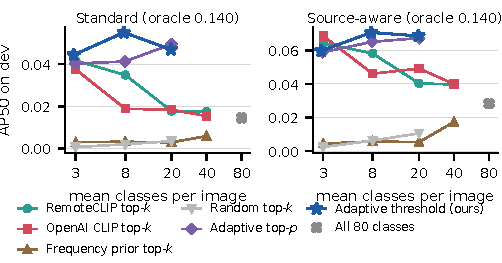
\includegraphics[width=\linewidth]{fig/dev_size_curve.pdf}
  \caption{Dev AP50 against the mean vocabulary size. Fixed top-$k$ selectors with CLIP encoders get worse as $k$ grows, the frequency prior and random lists stay near zero, and the adaptive rules (plotted at their mean size) are best at budgets of 8 and 20 classes.}
  \label{fig:devcurve}
\end{figure}

\cref{tab:dev} summarises the development stage and \cref{fig:devcurve} shows the effect of the budget.
For a fixed top-$k$, smaller is better: RemoteCLIP top-$k$ drops from 0.042 (\std) at $k=3$ to 0.018 at $k=20$, which agrees with the VocAda finding that more classes per noun reduce the gain \cite{liu2025vocada}.
At budgets of 8 and 20 classes the adaptive threshold is better than every fixed $k$ under both protocols, because it can spend a long prompt on an ambiguous image and a one-word prompt on a clear one; at a budget of 3 the fixed selectors are about as good.
OpenAI CLIP and RemoteCLIP are close at most fixed budgets, and RemoteCLIP is clearly ahead only at $k=8$.

The extensions were disappointing.
Local crop evidence improved the \emph{selection} of small-object classes (their recall at $k=8$ went from 0.22 to 0.31) but it did not improve detection: small-object recall went up while small-object AP went down, and the crops cost 83\,ms per image instead of 8\,ms.
Uncertainty retention showed the same pattern.
The caption selector cost about 1.2\,s per image on our GPU, more than three times the detector forward pass, and lost on class-averaged AP.
It won only on pooled F1, because captions often mention cars, which are the densest classes.
Synonym expansion tied on \src and lost on \std, so it failed the replacement rule we had fixed in advance and we kept the simpler method.

\subsection{Main result on the held-out test split}
\label{sec:exp_test}
\begin{table}[t]
  \centering
  \small
  \setlength{\tabcolsep}{4pt}
  \begin{tabular}{@{}lcccc@{}}
    \toprule
    Selector (test) & \#cls & AP50 \std & AP50 \src & vs.\ ours \\
    \midrule
    All 80 classes & 80 & 0.0053 & 0.0157 & robust \\
    Random (oracle size) & 2.3 & 0.0023 & 0.0038 & robust \\
    Frequency prior top-8 & 8 & 0.0028 & 0.0056 & robust \\
    OpenAI CLIP top-20 & 20 & 0.0081 & 0.0238 & robust (\std) \\
    RemoteCLIP top-8 & 8 & 0.0170 & 0.0347 & robust \\
    Adaptive threshold, $\sim$20 & 19.8 & 0.0209 & 0.0378 & n.s. \\
    Adaptive top-$p$, $\sim$20 & 19.8 & 0.0276 & 0.0406 & n.s. \\
    \textbf{Ours, $\sim$8} & 8.0 & \textbf{0.0280} & \textbf{0.0418} & -- \\
    \midrule
    \textit{Oracle} & 2.3 & 0.1072 & 0.1072 & -- \\
    \bottomrule
  \end{tabular}
  \caption{Results on the 2,862 held-out test images (single run, all settings frozen). ``robust'' means ours is better and all three checks agree under both protocols unless noted; n.s.\ = not significant.}
  \label{tab:test}
\end{table}

\cref{tab:test} is our main result.
Compared with the full vocabulary, the selector improves AP50 by +0.0228 under \std (basic CI $[+0.0143, +0.0263]$, 56 classes better against 18 worse, $p=1.1\times10^{-5}$) and by +0.0261 under \src (basic CI $[+0.0163, +0.0300]$, 50 against 24, $p=0.0034$).
The claim we declared before the run therefore holds under both protocols.
This is 22\% (\std) and 29\% (\src) of the oracle headroom.
On dev it was 38\%, so, as expected, the gain shrank somewhat once we stopped choosing the method on the same images.

For us the more interesting comparison is with RemoteCLIP top-8, which uses the \emph{same} encoder and the same average size.
Ours is robustly better under both protocols (+0.011 \std with 50/20 classes; +0.007 \src with 44/26), so the adaptive size really helps and the gain is not just a shorter prompt.
On dev this comparison had passed only two of the three checks, so the test set settled it.
The adaptive top-$p$ rule at about 20 classes is statistically tied with ours, which suggests that the per-image adaptation matters more than the exact budget.

\paragraph{F1.}
At the thresholds fixed on dev, F1 goes from 0.014 to 0.036 (\std) and from 0.039 to 0.056 (\src).
We should also report an awkward result for the metric: the frequency prior reaches a higher pooled F1 (0.084 / 0.132) while having almost the lowest AP.
Its fixed list is mostly FAIR1M vehicle classes plus xView ``Building'', which are the densest classes in the test split, and pooled F1 counts boxes while AP averages over classes.
We keep class-averaged AP as the headline, as declared before the run.

\begin{table}[t]
  \centering
  \small
  \setlength{\tabcolsep}{3.6pt}
  \begin{tabular}{@{}lcccccc@{}}
    \toprule
    & \multicolumn{3}{c}{AP50 \std} & \multicolumn{3}{c}{Recall@IoU0.5} \\
    \cmidrule(lr){2-4}\cmidrule(lr){5-7}
    Test, by object size & S & M & L & S & M & L \\
    \midrule
    All 80 classes & 0.002 & 0.005 & 0.011 & 0.05 & 0.21 & 0.47 \\
    RemoteCLIP top-8 & 0.004 & 0.014 & 0.037 & 0.08 & 0.25 & 0.50 \\
    \textbf{Ours} & \textbf{0.006} & \textbf{0.027} & \textbf{0.063} & \textbf{0.10} & \textbf{0.28} & \textbf{0.54} \\
    \midrule
    \textit{Oracle} & 0.052 & 0.129 & 0.197 & 0.41 & 0.67 & 0.88 \\
    \bottomrule
  \end{tabular}
  \caption{Test results by COCO object size (S $<32^2$, M $<96^2$ px, L otherwise). Selection helps every size, but small objects stay almost 10$\times$ below the oracle.}
  \label{tab:size}
\end{table}

\paragraph{Object size.}
\cref{tab:size} splits the test result by object size.
The relative gain is largest for medium and large objects (AP50 $\times$6.0 and $\times$5.9).
Small objects also improve, but they stay close to zero (0.006 against 0.052 for the oracle).
A tiling diagnostic on dev ($2{\times}2$ tiles plus the full image) did not raise small-object AP, lowered the overall AP of both the oracle (0.140 $\rightarrow$ 0.114) and our method (0.055 $\rightarrow$ 0.039), and was 5$\times$ slower, so we did not pursue it.

\subsection{Where does it work?}
\label{sec:exp_where}
\begin{figure*}[t]
  \centering
  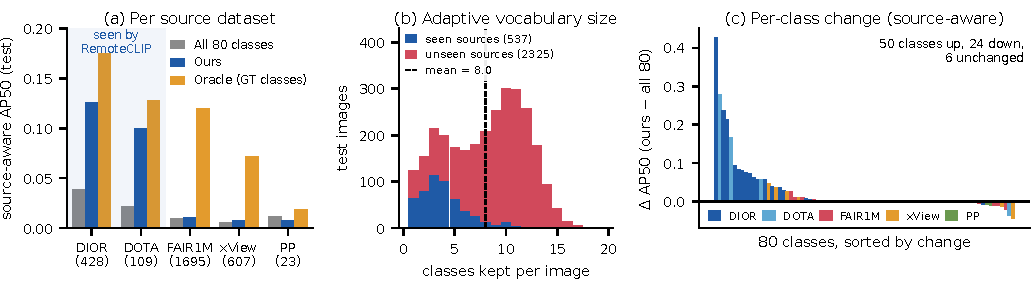
\includegraphics[width=\textwidth]{fig/test_analysis.pdf}
  \caption{Test-split analysis. (a) Source-aware AP50 per source dataset (number of test images in brackets); DIOR and DOTA are in RemoteCLIP's training data. (b) Number of classes kept per image by our frozen rule: images from the seen sources usually keep 1--7 classes, while FAIR1M/xView/PP images keep more. (c) Change in per-class AP50 against the full vocabulary, sorted and coloured by the source of the class.}
  \label{fig:test}
\end{figure*}

RemoteCLIP's training data contains DIOR and DOTA but not FAIR1M or xView \cite{liu2024remoteclip}, so before the test run we fixed a split of \lae sources into a seen group (DIOR, DOTA) and an unseen group (FAIR1M, xView, PP).
\cref{fig:test}a shows that the gain is almost entirely on the seen group: source-aware AP50 rises from 0.035 to 0.120 there (3.5$\times$; 20 of 23 classes better, $p=5\times10^{-4}$), whereas on the unseen group it moves from 0.008 to 0.009 (not significant) although the oracle shows about 11$\times$ headroom.
The vocabulary sizes in \cref{fig:test}b tell the same story from the selector's side.
On seen sources RemoteCLIP is confident and keeps 4.0 classes on average (27\% of these images keep one or two), while on unseen sources it spreads its probability and keeps 8.9.
The per-class view (\cref{fig:test}c) is consistent: the large gains are DIOR and DOTA classes, the FAIR1M and xView classes cluster around zero, and the 24 classes that lose, lose very little.

\begin{table}[t]
  \centering
  \small
  \setlength{\tabcolsep}{4pt}
  \begin{tabular}{@{}lccc@{}}
    \toprule
    NWPU VHR-10 (614 images) & \#cls & AP50 & $\Delta$ vs.\ all 80 \\
    \midrule
    All 80 classes & 80 & 0.088 & -- \\
    RemoteCLIP top-8 & 8 & 0.093 & +0.005 (n.s.) \\
    OpenAI CLIP top-20 & 20 & 0.100 & +0.012 (robust) \\
    \textbf{Ours (frozen $t$)} & 3.9 & \textbf{0.129} & \textbf{+0.041} (robust) \\
    \midrule
    \textit{Oracle} & 1.4 & 0.208 & +0.120 \\
    \bottomrule
  \end{tabular}
  \caption{Transfer to NWPU VHR-10 with every method frozen and no recalibration. Standard and source-aware AP are identical here.}
  \label{tab:nwpu}
\end{table}

\paragraph{External data.}
On NWPU VHR-10, applied without any retuning, our selector improves AP50 from 0.088 to 0.129 (+0.041, CI $[+0.030, +0.057]$, 8 of 9 classes better), while fixed-size RemoteCLIP top-8 gives no significant gain (\cref{tab:nwpu}).
The frozen threshold keeps only 3.9 classes per image here, because RemoteCLIP is more confident on these DIOR-like images, and this is exactly where a fixed $k$ cannot follow.
Most of the gain comes from two classes, ground track field (0.007 $\rightarrow$ 0.243) and vehicle (0.000 $\rightarrow$ 0.163), while airplane, which the full prompt already detects, loses 0.07.
We want to be careful about what this shows.
NWPU was made by the same group as DIOR with DIOR's class names, and LAE-1M even includes it as a training source \cite{pan2025lae}.
So this is transfer to new images of a \emph{familiar} kind, not a general unseen-domain result.
We also could not check image overlap between NWPU and the DIOR training images that RemoteCLIP used.

\subsection{Speed}
On the RTX 5060 (GPU idle, fp32, 200 dev images, 3 passes, selector and detector in the same process) the median end-to-end time is 414\,ms with all 80 classes and 343\,ms with ours, including 7.9\,ms for the selector.
That is 1.21$\times$ faster (difference $-71$\,ms, CI $[-72, -71]$), and peak GPU memory also drops from 2.77 to 2.49\,GB.
The saving comes from the detector itself (414 $\rightarrow$ 335\,ms), as a shorter prompt means less text in the fusion layers, which is related to the cost of long prompts that WeDetect describes for fusion detectors \cite{fu2026wedetect}.
For reference, VocAda reports 5.6--10.7\,s per image on a V100 \cite{liu2025vocada}, but with a different detector, so it is not a direct comparison.

\subsection{Failure analysis}
\label{sec:exp_fail}
\begin{figure*}[t]
  \centering
  \begin{subfigure}{0.325\textwidth}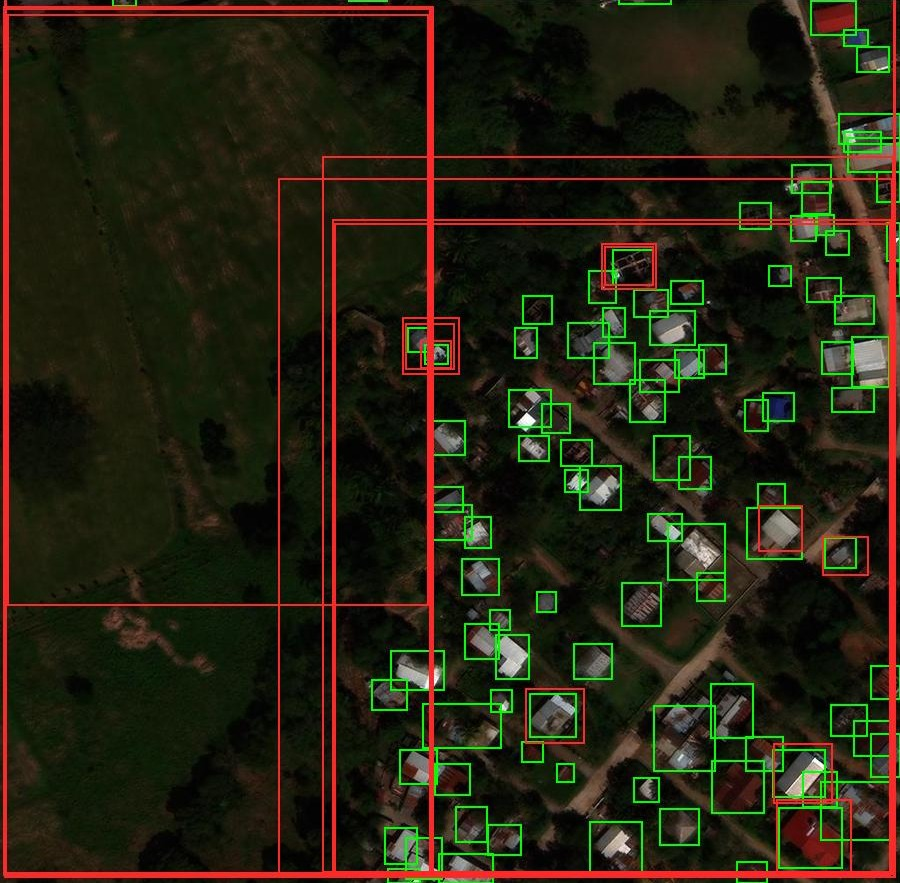
\includegraphics[width=\linewidth]{fig/qual_full.jpg}\caption{All 80 classes}\end{subfigure}\hfill
  \begin{subfigure}{0.325\textwidth}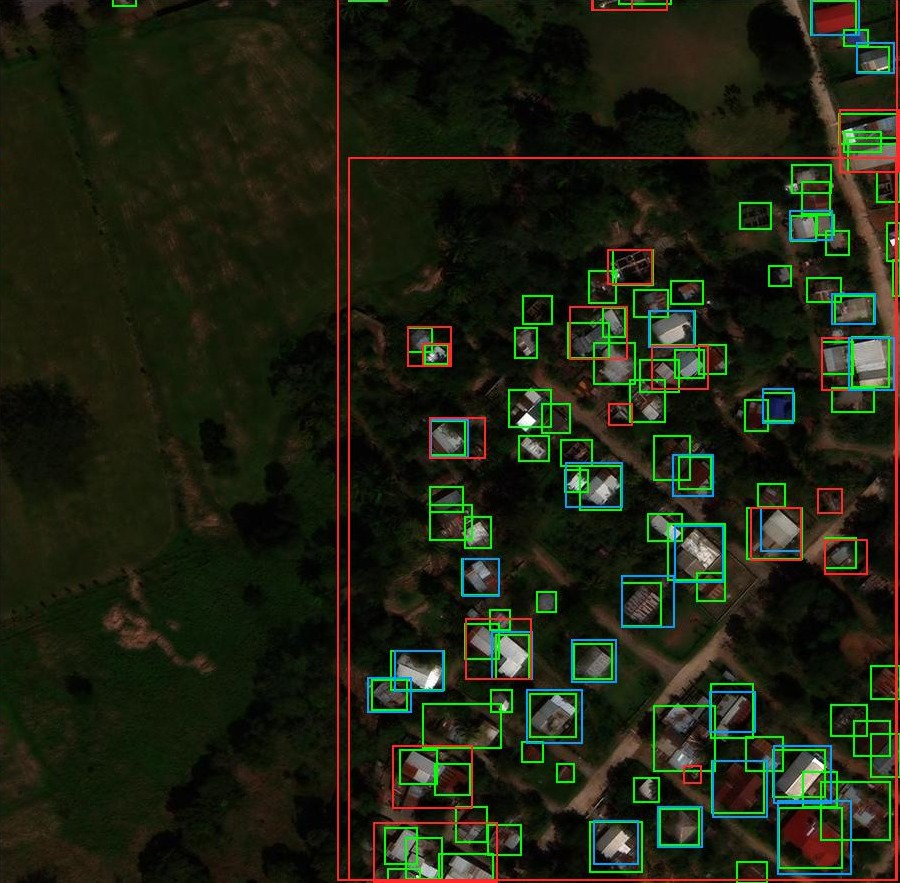
\includegraphics[width=\linewidth]{fig/qual_ours.jpg}\caption{Ours, same image}\end{subfigure}\hfill
  \begin{subfigure}{0.325\textwidth}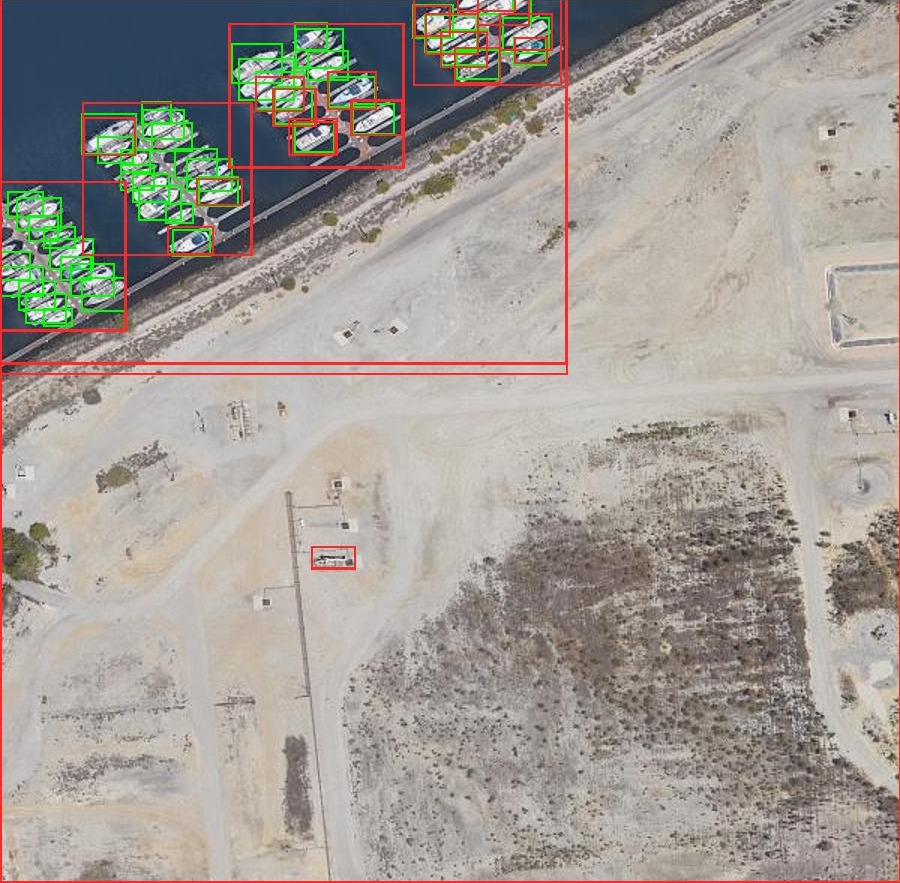
\includegraphics[width=\linewidth]{fig/qual_fail.jpg}\caption{Failure: near-synonym classes}\end{subfigure}
  \caption{Qualitative results on dev images, chosen by fixed rules and not by hand. (a, b) xView village (image 3229), the image with the largest true-positive gain of ours over the full prompt: the full prompt produces huge false boxes, our vocabulary recovers many buildings. (c) FAIR1M marina (image 2154), the image with the most wrong-class outcomes for our method: the boats are boxed well but receive a different class name. Green = ground truth, blue = true positive, red = false positive at score $\geq0.14$.}
  \label{fig:qual}
\end{figure*}

We sorted every labelled object and every confident detection on the dev images into failure types that we had defined before looking at them.
The main findings are listed below, and \cref{fig:qual} shows one success and one failure.
\begin{itemize}
  \item Our selector keeps the right class for only 26\% of ground-truth \emph{objects}, because images with more than 20 objects hold 85\% of all objects, and on FAIR1M and xView it keeps the right class for only 22\% and 24\% of the objects.
  \item 59\% of the selected classes belong to another source's label set, \eg xView ``Ferry'' on a FAIR1M image labelled ``Passenger Ship''. This is the hard-negative problem of \cite{bianchi2024devil} and the overlapping-concept problem of \cite{li2024lbp}, here produced by the benchmark taxonomy. A diagnostic that restricts the selection to the true source raises object coverage from 0.25 to 0.68, but it needs the source label, which a deployable selector does not have.
  \item When the right class \emph{is} kept, \gdino finds 48\% of those objects, against 58\% with the oracle, so in that case the detector behaves almost as if it had the perfect vocabulary.
  \item Confident detections drop by 76\% (28,580 $\rightarrow$ 6,747) and their true-positive share triples (0.008 $\rightarrow$ 0.027). With all 80 classes, 77\% of the confident detections are classes never annotated in that image's dataset.
  \item Selection helps sparse scenes (1--5 objects: 0.025 $\rightarrow$ 0.109 AP50) but hurts scenes with more than 20 objects (0.038 $\rightarrow$ 0.017 for 21--100 objects).
  \item Rare classes stay near zero for every vocabulary, the oracle included (0.050), so better selection cannot rescue them.
\end{itemize}

\section{Limitations}
\label{sec:limits}
% HR: reviewers will ask these anyway so better we say them first
\begin{itemize}
  \item Absolute numbers are low. Even with a perfect vocabulary the frozen \gdino-T reach only 0.107 AP50 on test, and some classes stay near zero.
  \item The gain is limited to imagery and label spaces close to RemoteCLIP's training data.
  \item One detector (Swin-T) and one benchmark family. We did not test bigger detectors like \gdino-B or OWLv2. \TODO{if time / compute allows}
  \item The rule family and the target size of 8 were designed by us on dev, and the synonym experiment was motivated by our own dev failure analysis. Both were frozen before test but readers should know.
\end{itemize}

\section{Conclusion}
\label{sec:conclusion}
% TODO: rewrite, this is just placeholder text from the meeting
We showed that choosing a small per-image vocabulary from pixels, with an aerial CLIP model and a calibrated adaptive size, robustly improves a frozen open-vocabulary detector on held-out aerial images at almost no cost.
The benefit is real but bounded: it holds where the encoder knows the imagery, and it is capped by near-synonym classes across merged datasets and by the detector on small objects.
\TODO{future work: taxonomy-aware vocabularies, aerial-adapted detector, other OVD models}


{
    \small
    \bibliographystyle{ieeenat_fullname}
    \bibliography{main}
}

\end{document}
